\section{Introduction}
\label{sec:intro}


A surveillance task for the gas emission monitoring includes sensing coverage to detect gas leaks and building a gas distribution model to accurately locate the gas concentrations in the environment. This information can be useful to make better strategic decisions in order to mitigate the gas emissions.



We perform the gas emission monitoring task using a mobile robot equipped with a spectroscopy-based remote gas sensor (Fig.~\ref{fig:gasbot}). 
In particular, we use a Tunable Diode Laser Absorption Spectroscopy (TDLAS), which can collect integral concentrations along the line-of-sight.
In our setup, the remote gas sensor installed on the mobile robot is actuated using a pan-tilt unit.
This means it can project optical beams in different directions, and therefore, a large circular sector can be sampled at a particular pose in the environment, which we referred as a \textit{sensing configuration} ($c$). 



%*******************************************************************
%/////////// Fig: (a) Gasbot (b) Sensing configuration 
%*******************************************************************
% --- Gasbot / Sensing configuration ----
\begin{figure}[ht!]
	\begin{center}	
		\vspace{2em}	
		% --- Gasbot ---
		\subfigure[A gas-sensitive mobile robot]{\label{fig:gasbot}		
		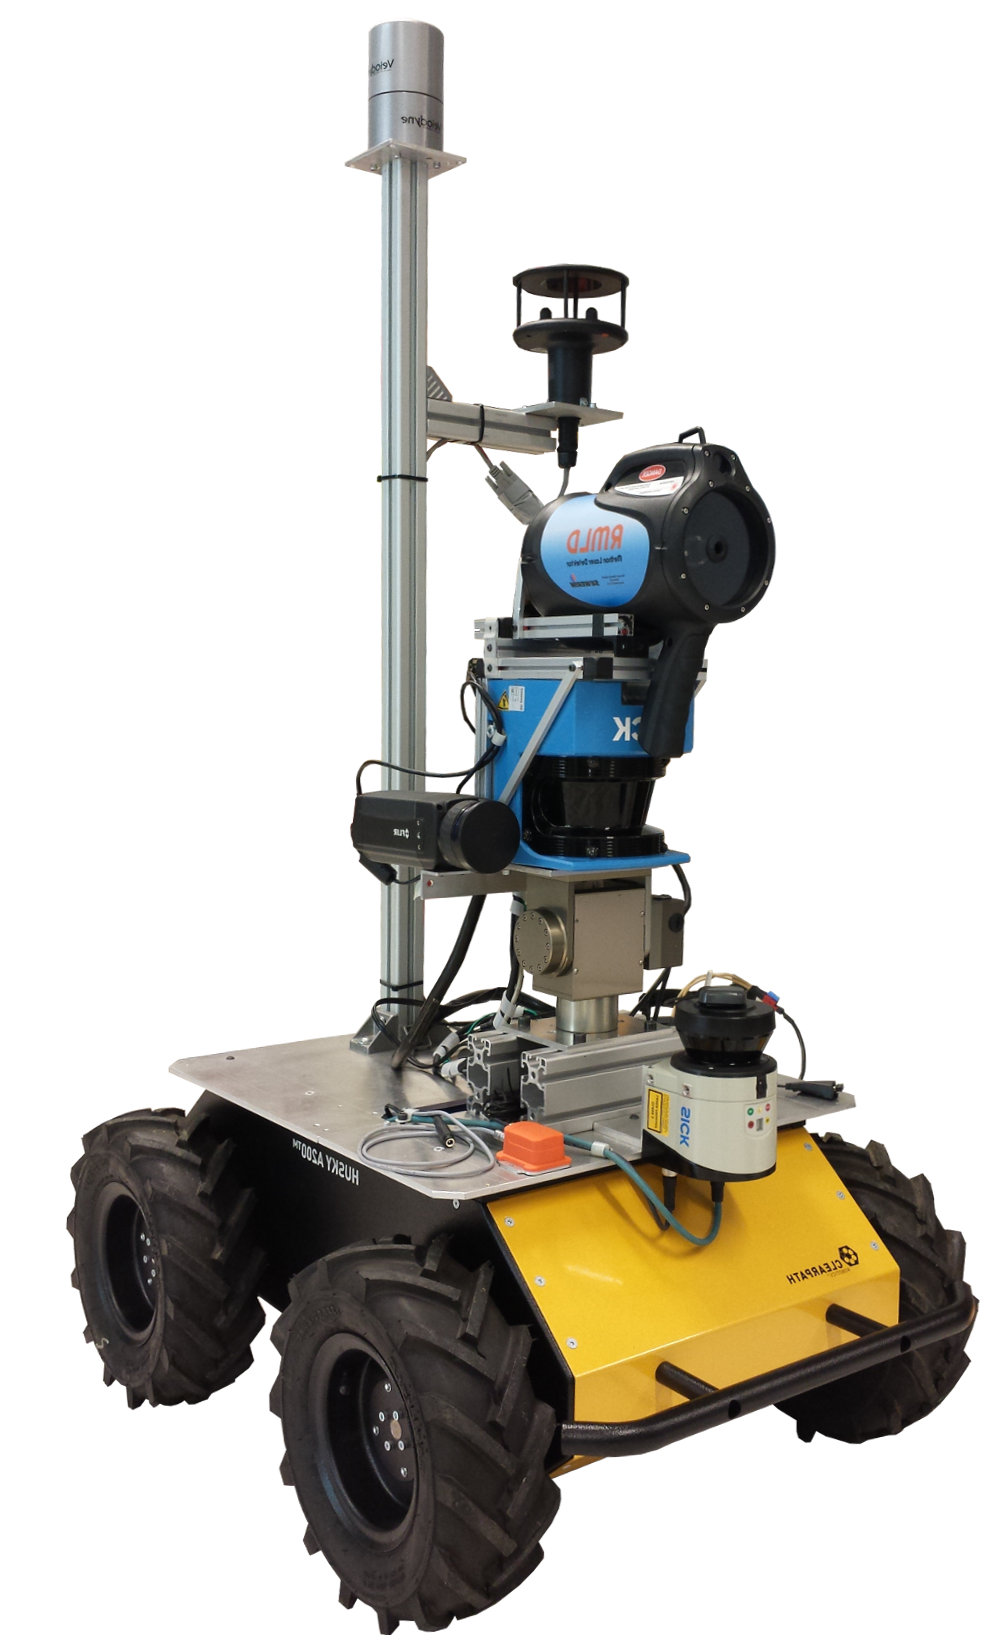
\includegraphics[width=2.5cm]{fig/gasbot.png}}
		% --- TDLAS measurement ---
		\begin{picture}(0,0)
		\put(118,-178){
			\put(-135,230){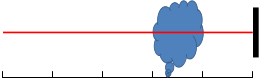
\includegraphics[width=5cm]{fig/RMLD_WorkingPrinciple.png}}
			\small
			\put(-127,272){\FramedBox{0.5cm}{2.5cm}{\textcolor{red}{\small 1200 ppm $\times$ m}}}
			\put(-127,305){\cfbox{white}{\rotatebox{0}{{\tabular[t]{@{}c@{}}Background \\concentration: \\ 200 ppm $\times$ m \endtabular}}}}		
			\put(-060,305){\cfbox{white}{\rotatebox{0}{{\tabular[t]{@{}c@{}}Gas source \\concentration: \\1000 ppm $\times$ m \endtabular}}}}
			\put(-135,220){0}
			\put(-108,220){1}
			\put(-081,220){2}
			\put(-054,220){3}
			\put(-027,220){4}
			\put( 002,220){5 m}}
		\end{picture}
		\hspace{15em}
		% --- Sensing Conf ---
		\subfigure[Sensing configuration]{\label{fig:conf}
		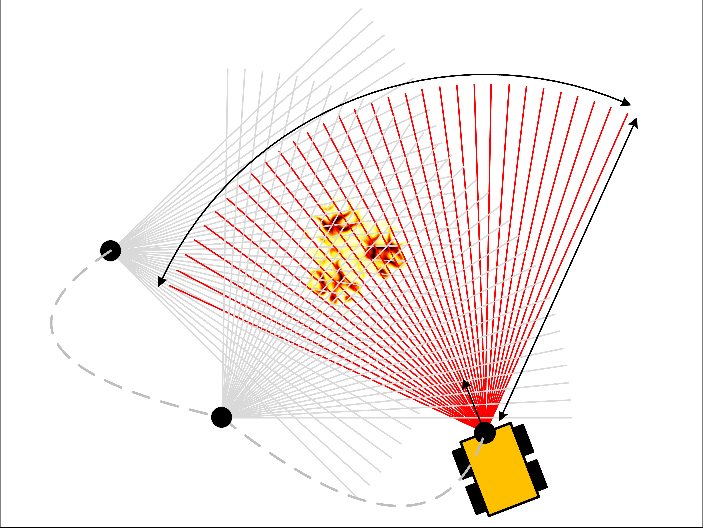
\includegraphics[trim={5 5 5 5}, clip,width=6cm,angle=0,origin=c]{fig/gas_tomography.pdf}}
		\begin{picture}(0,0)
		\normalsize
		\put(60,10){
			\put(-090,050){$r$}
			%\put(-165,008){$<x,y,\theta>$}
			\put(-155,008){$(x,y,\theta)$}
			\put(-160,095){$\phi$}
			\put(-222,055){$c_1$}
			\put(-192,008){$c_2$}
			\put(-102,009){$c_3$}}
		\end{picture}
		\caption{ 
		(a) The robot is equipped with an actuated TDLAS sensor, which reports integral concentration of methane along its line-of-sight.
		(b) A sensing configuration $c$ is sampling a circular sector ($r,\phi$) by emitting $s$ optical beams at pose $(x,y,\theta)$.
		}
	\end{center}
	%\vspace{-2em}
\end{figure}


%*******************************************************************

A robotic solution for the surveillance task is a tour of selected sensing configurations $\{c_1,c_2,..,c_n\}$to sample the environment. An efficient plan consists of least number of sensing configurations and minimum traveling distance, and yet provides a surveillance that result into maximum sensing coverage and high quality reconstructions of gas distribution. % between the configurations are minimized so that the overall sensing are least environment is sampled
%Our sensing planning algorithm provides an efficient sensing coverage in this regard.

%** We define sensing configuration as collecting integral measurements within a circular sector ($r,\phi$) by measuring along $s$ equally spaced beams of length $r$ inside the field of view $\phi$ at pose ($x, y, \theta$), see Fig.~\ref{fig:conf}. **

